%==============================================================================
%  Projektarbeit – Just-in-Time-Privilege-Elevation
%
%  Kompilieren:  pdflatex Projektarbeit.tex  (zweimal, wegen Inhaltsverzeichnis)
%  Schrift:      Latin Modern, 11pt, 1,5-zeilig
%  Klasse:       KOMA-Script (scrartcl)
%
%  Anpassen: Titelblock unten (Autor, Matrikelnummer, Betreuer, Hochschule).
%==============================================================================
\documentclass[11pt,a4paper]{article}

% --- Kodierung & Sprache -----------------------------------------------------
\usepackage[T1]{fontenc}
\usepackage[utf8]{inputenc}
\usepackage[ngerman]{babel}

% --- Schrift & Mikrotypografie ----------------------------------------------
\usepackage{lmodern}
\usepackage{microtype}     % feiner Randausgleich, Zeichenskalierung

% --- Seitenlayout ------------------------------------------------------------
\usepackage[
  left=3cm, right=2.5cm, top=2cm, bottom=2cm,
]{geometry}
\usepackage{setspace}
\setstretch{1.22}          % leicht reduzierter Zeilenabstand (Platzgründe)
\usepackage{parskip}       % Absatzabstand statt Erstzeilen-Einzug
\setlength{\parskip}{0.3\baselineskip}

% --- Kopf-/Fußzeile ----------------------------------------------------------
\usepackage{fancyhdr}
\pagestyle{fancy}
\fancyhf{}
\fancyhead[L]{\small Just-in-Time-Privilege-Elevation}
\fancyhead[R]{\small\thepage}
\renewcommand{\headrulewidth}{0.4pt}

% --- Tabellen, Grafiken, Beschriftungen -------------------------------------
\usepackage{booktabs}
\usepackage{graphicx}
\usepackage{float}
\usepackage{flafter}           % Floats erscheinen nie vor ihrer Referenz
\usepackage{caption}
\captionsetup{font=small,labelfont=bf}
\raggedbottom                  % kein gestreckter Leerraum am Seitenende

% --- Farben ------------------------------------------------------------------
\usepackage{xcolor}

% --- Kompaktere Überschriften-Abstände (Platzgründe) ------------------------
\makeatletter
\renewcommand\section{\@startsection{section}{1}{\z@}%
  {-2.3ex \@plus -1ex \@minus -.2ex}{1.2ex \@plus .2ex}%
  {\normalfont\Large\bfseries}}
\renewcommand\subsection{\@startsection{subsection}{2}{\z@}%
  {-1.8ex \@plus -1ex \@minus -.2ex}{0.8ex \@plus .2ex}%
  {\normalfont\large\bfseries}}
\makeatother

% --- Hyperlinks (dezent, druckfreundlich) -----------------------------------
\usepackage[hidelinks]{hyperref}

%==============================================================================
\begin{document}

%------------------------------------------------------------------ Titelseite
\begin{titlepage}
  \centering
  {\scshape\large Methoden und Werkzeuge der Softwareentwicklung\par}
  \vspace{0.5cm}
  {\scshape Projektarbeit\par}
  \vfill
  {\Huge\bfseries Just-in-Time-Privilege-Elevation\par}
  \vspace{0.8cm}
  {\Large Ein Modul für zeitlich befristete,\\[0.2em]
   zwei-faktor-gesicherte Rechte-Erhöhung\par}
  \vfill
  \begin{tabular}{rl}
    Autor:        & Lukas Cvitanović \\        % <- anpassen
    Matrikelnr.:  & \rule{4cm}{0.4pt} \\        % <- anpassen
    Kurs:         & \rule{4cm}{0.4pt} \\        % <- anpassen
    Betreuer:     & \rule{4cm}{0.4pt} \\        % <- anpassen
  \end{tabular}
  \vspace{1.5cm}

  {\large \today\par}
\end{titlepage}

%--------------------------------------------------------- Inhaltsverzeichnis
\tableofcontents
\clearpage

%==============================================================================
\section{Einleitung und Motivation}

Administrative Berechtigungen werden in vielen Systemen dauerhaft vergeben:
Ein Konto besitzt erhöhte Rechte unabhängig davon, ob diese im Moment benötigt
werden. Das widerspricht dem Least-Privilege-Prinzip~\cite{owasp_polp}, vergrößert
den Schaden einer Kontoübernahme, da ein kompromittiertes Administratorkonto jederzeit
voll handlungsfähig ist, und erschwert die Nachvollziehbarkeit. Als Antwort hat
sich \emph{Just-in-Time}-Zugriff (JIT) etabliert: Rechte werden nur für den
konkreten Bedarfsmoment gewährt und laufen automatisch ab. Der Zeitraum für
möglichen Missbrauch sinkt auf wenige Minuten, und jede Erhöhung wird zu einem
protokollierbaren Ereignis.

Die vorliegende Arbeit entwirft und implementiert ein eigenständiges,
wiederverwendbares Modul, das JIT-Privilege-Elevation als Bibliothek
bereitstellt, vom Trägersystem entkoppelt ist und beispielhaft in eine
bestehende PaaS-Umgebung integriert wird. Es folgen Anforderungen
(Abschnitt~2), Stand der Technik (3), Konzept (4), Sicherheitsanalyse nach
STRIDE (5), Implementierung (6) und Evaluation (7).

%==============================================================================
\section{Anforderungen}

\textbf{Funktional:} Ein Benutzer kann eine zeitlich befristete
Rechte-Erhöhung \emph{beantragen}, die erst nach erneuter
Zwei-Faktor-Bestätigung (Step-Up-Authentication) wirksam wird. Aktive
Erhöhungen lassen sich vorzeitig widerrufen und laufen andernfalls automatisch
ab; jeder Schritt wird manipulationssicher protokolliert.

\textbf{Nicht-funktional:} \emph{Fail-closed}, das heißt im Zweifel oder bei
jedem Fehler wird kein Recht gewährt; \emph{Unabhängigkeit} vom Trägersystem
(Ports-and-Adapters); \emph{Nachvollziehbarkeit} durch einen lückenlosen,
integritätsgesicherten Audit-Trail; \emph{Korrektheit}, verifiziert durch
automatisierte Tests inklusive Nebenläufigkeit.

%==============================================================================
\section{Stand der Technik}

Verfahren zur kontrollierten Rechteerhöhung sind etabliert und unterscheiden
sich vor allem in Granularität und Betriebsaufwand (Tabelle~\ref{tab:sota}).
Während Vault~\cite{vault}, Boundary~\cite{boundary} bzw.\
Teleport~\cite{teleport} und OIDC-Provider wie Keycloak~\cite{keycloak} eigene
Infrastruktur bzw.\ hohen Betriebsaufwand voraussetzen, verfolgt das hier
entwickelte Modul einen leichtgewichtigen Ansatz: Es führt die Erhöhung als
eingebettete Bibliothek statt als externe Infrastruktur durch und bleibt durch
das Ports-and-Adapters-Muster~\cite{hexagonal} unabhängig vom Trägersystem.

\begin{table}[htbp]
  \centering
  \caption{Einordnung verwandter Systeme}
  \label{tab:sota}
  \begin{tabular}{@{}lll@{}}
    \toprule
    \textbf{System} & \textbf{Ansatz} & \textbf{Abgrenzung} \\
    \midrule
    HashiCorp Vault (SSH)      & kurzlebige SSH-Zertifikate     & OS-Ebene, eigene Infrastruktur \\
    Boundary / Teleport        & Session-Broker mit Recording   & mächtig, hoher Betriebsaufwand \\
    Keycloak / Authentik       & OIDC-basierte Re-Auth          & Identity-Provider-zentriert \\
    \textbf{Dieses Modul}      & eingebettete JIT-Erhöhung      & leichtgewichtig, integrierbar \\
    \bottomrule
  \end{tabular}
\end{table}

%==============================================================================
\section{Konzept und Architektur}

\subsection{Einordnung in die Bestandsarchitektur}
Abbildung~\ref{fig:arch} zeigt die Integration in eine typische
DEV/PROD-Topologie. Grau dargestellt ist der Status quo: zwei gleichwertige,
vollständige Stacks (Entwicklung und Produktion) aus jeweils Frontend, Backend
und Datenbank sowie der Deploy-Pfad über das Git-Repository. Farbig
hervorgehoben ist die Ergänzung durch das vorgestellte Modul: Der Benutzer
beantragt beim JITPE-Dienst eine zeitlich befristete Erhöhung und bestätigt sie
per Zweitfaktor. \emph{Beide} Umgebungen behandeln JITPE identisch -- vor jeder
privilegierten Aktion fragt das jeweilige Backend dort nach (\emph{verify}); nur
bei aktiver Erhöhung wird die Aktion ausgeführt, andernfalls verweigert
(fail-closed). Intern folgt das Modul dem Ports-and-Adapters-Muster: Der Kern
kennt das Host-System nicht, sondern spricht ausschließlich gegen Interfaces
(siehe Abschnitt~6).

\begin{figure}[htbp]
  \centering
  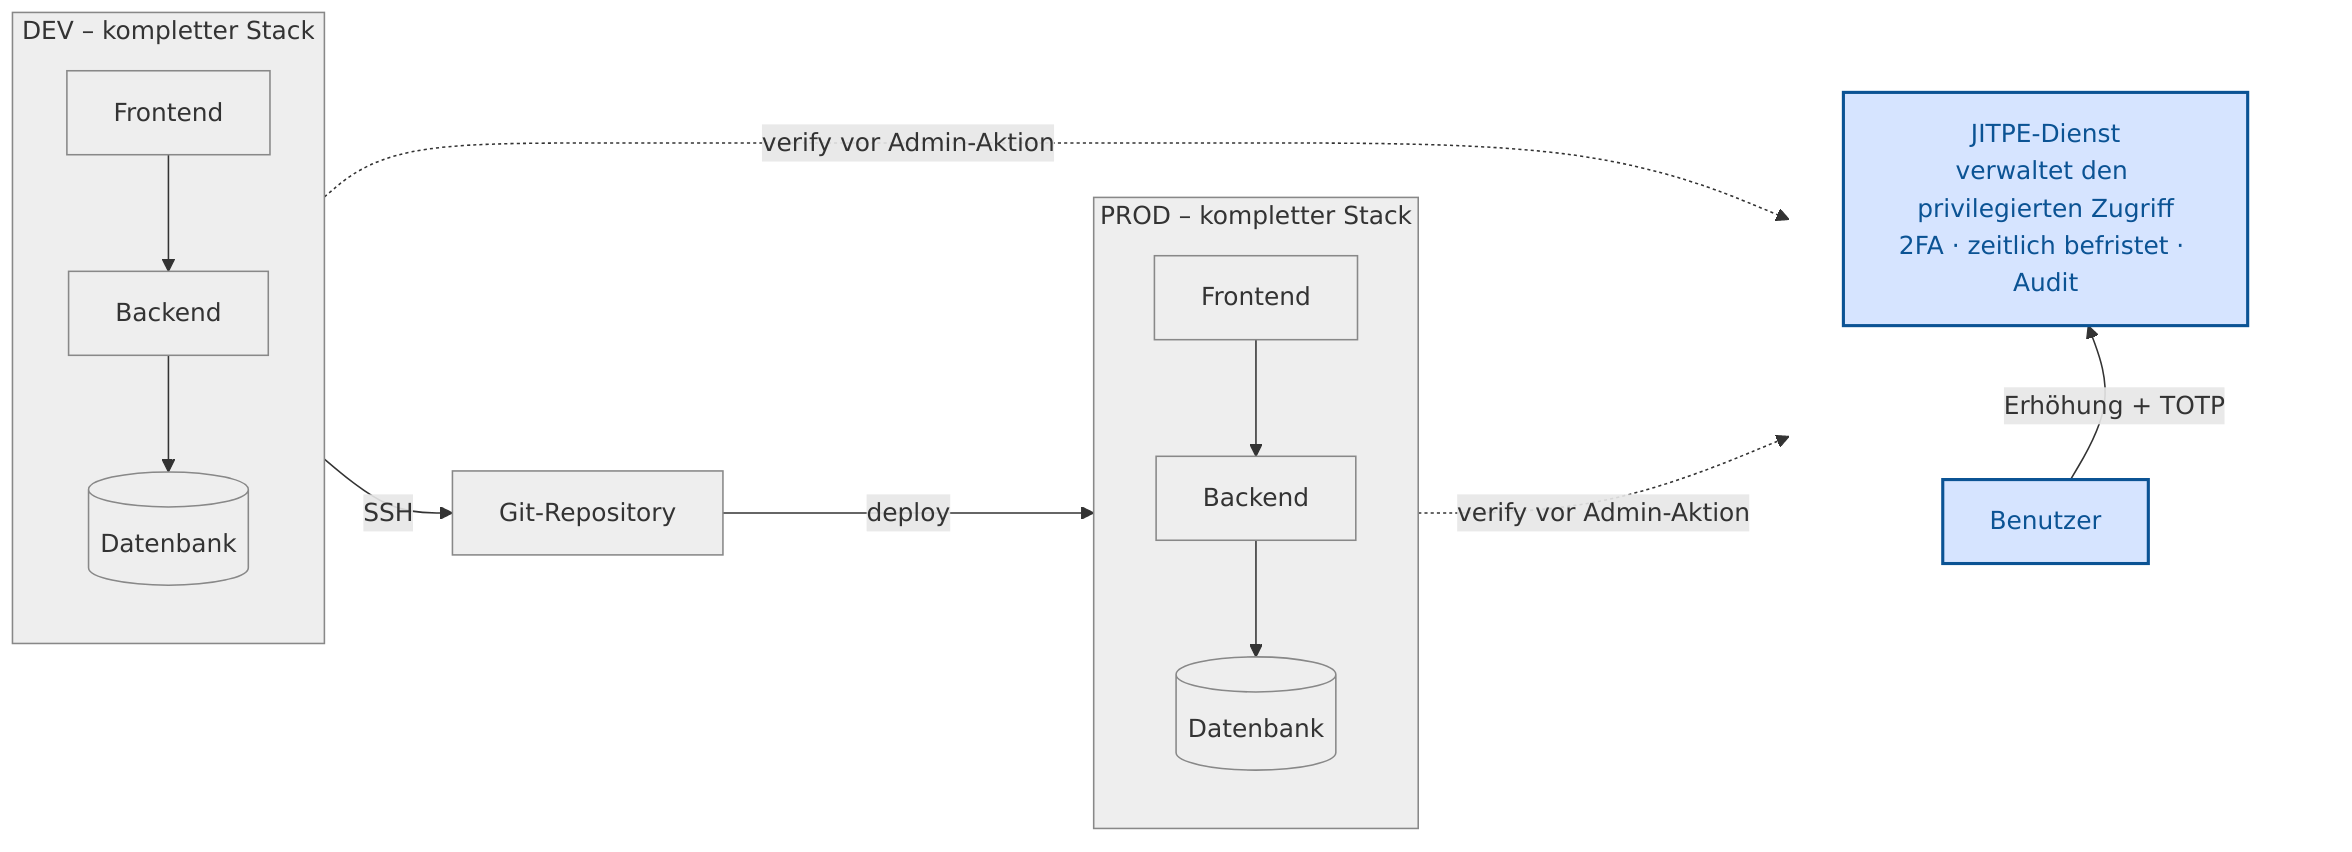
\includegraphics[width=\textwidth]{figures/arch.png}
  \caption{Integration: DEV und PROD (Status quo, grau) sind gleichwertige
    Stacks; beide fragen das JITPE-Modul (blau) identisch vor jeder
    privilegierten Aktion (\emph{verify})}
  \label{fig:arch}
\end{figure}

\subsection{Lebenszyklus, Ablauf und Datenmodell}
Eine Rechte-Erhöhung (Grant) durchläuft die Zustände \texttt{pending} (Antrag
gestellt), \texttt{active} (per TOTP bestätigt) und schließlich einen der
terminalen Zustände \texttt{expired}, \texttt{revoked} oder \texttt{denied}.
Alle Endzustände sind terminal; ein abgelaufener, widerrufener oder abgelehnter
Grant wird nie wieder aktiv (fail-closed). Der Ablauf umfasst damit vier Phasen:
Antrag, Bestätigung per TOTP (Step-Up; ohne gültigen zweiten Faktor keine aktive
Erhöhung), Nutzung der geschützten Aktion und automatischer Ablauf durch einen
Hintergrund-Ticker. Persistiert wird dies in drei Tabellen:
den Grants, dem Audit-Log und einer Tabelle der bereits verbrauchten
TOTP-Zeitfenster für den benutzerweiten Replay-Schutz. Die Audit-Tabelle bildet
eine Hash-Kette: Jeder Eintrag enthält den SHA-256-Hash~\cite{fips180} seines
Vorgängers, sodass jede nachträgliche Manipulation die Kette am Folgeeintrag
bricht.

%==============================================================================
\section{Sicherheitsanalyse}

Die Analyse folgt STRIDE~\cite{msstride} und ordnet jeder Bedrohung eine
konkrete Gegenmaßnahme im Entwurf bzw.\ im Code zu. Annahmen: Der Host authentifiziert die
Primäridentität, TLS sichert die Transportwege (Browser/Backend und
Backend/Datenbank), und der TOTP-Seed liegt verschlüsselt im Secret-Store und
verlässt ihn nie im Klartext.

\subsection{Bedrohungsklassen}
Jede Klasse ist im Code verortet: \emph{Spoofing} scheitert am TOTP-Step-Up;
\emph{Tampering} an der SHA-256-Hash-Kette (\texttt{audit.go}); \emph{Repudiation}
am lückenlosen, pflichtigen Protokoll; \emph{Information Disclosure} an
verschlüsselten Seeds (AES-256-GCM~\cite{nistgcm}) und 128-Bit-Zufalls-IDs. Die Kernklasse
\emph{Elevation of Privilege} wird mehrfach abgesichert: Die \texttt{PolicyEngine}
deckelt Rolle und Dauer, ein Ticker erzwingt den Ablauf (\texttt{ExpireDue}), die
Aktivierung ist atomar gegen Doppel-Erhöhung, und die Autorisierung erfolgt
serverseitig und fail-closed (\texttt{Check}). Einzig \emph{Denial of Service}
ist kein Gewinn (siehe unten).

\subsection{Vergleich mit dem Grundsystem}
Tabelle~\ref{tab:vergleich} stellt die Klassen dem Grundsystem gegenüber, dem
üblichen Zugriff über dauerhafte SSH-Schlüssel und stehendes \texttt{sudo}. In
fünf der sechs Klassen ist das Modul überlegen; nur bei der Verfügbarkeit (D)
ist fail-closed ein bewusster Trade-off zugunsten der Sicherheit. Kernunterschied:
Privileg ist im Grundsystem der Dauerzustand, im Modul die befristete, geprüfte
Ausnahme.

\begin{table}[htbp]
  \centering
  \caption{JIT-Modul gegenüber dem Grundsystem (dauerhafte Schlüssel + sudo)}
  \label{tab:vergleich}
  \small
  \renewcommand{\arraystretch}{1.25}
  \begin{tabular}{@{}p{3.3cm}p{5.0cm}p{4.9cm}@{}}
    \toprule
    \textbf{Klasse} & \textbf{Grundsystem} & \textbf{JIT-Modul} \\
    \midrule
    Spoofing          & ein Schlüssel, unbefristet gültig    & zwei Faktoren, 30-s-TOTP mit Replay-Schutz \\
    \addlinespace[4pt]
    Tampering         & Log lokal und veränderbar            & zentrale, verkettete Hash-Sicherung \\
    \addlinespace[4pt]
    Repudiation       & Login ohne Begründung                & Akteur + Pflicht-Begründung, unveränderlich \\
    \addlinespace[4pt]
    Info Disclosure   & Key-Leak = Dauerzugriff              & kurzlebiger Grant, kein Langzeitgeheimnis \\
    \addlinespace[4pt]
    Denial of Service & bei Ausfall verfügbar                & fail-closed (bewusster Trade-off) \\
    \addlinespace[4pt]
    Elevation         & Privileg ist Dauerzustand            & Privileg ist befristete, geprüfte Ausnahme \\
    \bottomrule
  \end{tabular}
\end{table}

\subsection{Quantitativer Angriffsaufwand}
Der Vorteil lässt sich beziffern (Tabelle~\ref{tab:zahlen}). Der Rechenweg ist
für alle Brute-Force-Werte identisch:
\[
  t \;=\; \frac{\mathrm{Suchraum}}{(\mathrm{Versuche/Sekunde}) \;\cdot\; 3{,}15\cdot10^{7}\,\mathrm{s/Jahr}}.
\]
Für den verschlüsselten TOTP-Seed (AES-256) etwa ergibt sich bei optimistischen
$10^{18}$ Versuchen/s: $t = 2^{256}/(10^{18}\cdot 3{,}15\cdot10^{7}) \approx
3{,}7\cdot10^{51}$ Jahre. Der entscheidende Punkt ist nicht nur die Größe der
Räume, sondern die \emph{Rotation}: Da der TOTP-Code alle 30\,s wechselt und je
Antrag nur ein Versuch möglich ist (ein falscher Code verwirft den Antrag),
akkumuliert ein Angreifer keinen Fortschritt -- anders als beim statischen
Geheimnis des Grundsystems.

\begin{table}[htbp]
  \centering
  \caption{Aufwand für dauerhaften Admin-Zugang (Annahme: Primitive sicher)}
  \label{tab:zahlen}
  \small
  \renewcommand{\arraystretch}{1.25}
  \begin{tabular}{@{}p{3.6cm}p{4.6cm}p{4.9cm}@{}}
    \toprule
    \textbf{Angriff} & \textbf{Grundsystem} & \textbf{JIT-Modul} \\
    \midrule
    Dauer-Geheimnis knacken & 1 statischer Hash, endlich (Sek.\ bis Tage) & AES-256-Seed: $2^{256}\!\approx\!10^{51}$ Jahre \\
    \addlinespace[4pt]
    ID/Token erraten        & ---                                          & $2^{128}\!\approx\!1{,}1\cdot10^{22}$ Jahre \\
    \addlinespace[4pt]
    Code online raten       & statisch, kumulativ                          & $10^{6}$, nur 1 Versuch je Antrag \\
    \addlinespace[4pt]
    Lebensdauer gestohlenes Geheimnis & unbegrenzt                         & $\le 30$ min (dann \texttt{expires\_at}) \\
    \bottomrule
  \end{tabular}
\end{table}

\subsection{Fail-closed als durchgängiges Prinzip}
Jeder Fehlerpfad, sei es ein Policy-Fehler, fehlender oder falscher TOTP,
Replay, abgelaufene Frist oder Store-Fehler, führt zu keinem aktiven Grant.
\texttt{Check} liefert im Zweifel \texttt{false}. Dies ist durch Tests belegt
(u.\,a. \texttt{TestCheck\_FailsClosedOnStoreError}).

%==============================================================================
\section{Implementierung}

\subsection{Modul-Struktur}
Das Modul ist in Go geschrieben und besteht aus dem Kern (Domänentypen,
State-Machine, die Schnittstellen in \texttt{ports.go}, die Hash-Kette in
\texttt{audit.go}, eine Beispiel-Policy sowie die zentrale Logik in
\texttt{module.go}) und zwei Adaptern: einem In-Memory-Store und einem
TOTP-Verifier nach RFC~6238. Der Kern hat keine externen Abhängigkeiten.

\subsection{Die Schnittstellen (Ports)}
Der Kern definiert fünf Schnittstellen, die das Host-System implementiert. Die
zentrale ist \texttt{Store} für die Persistenz: Sie umfasst das Anlegen und
Lesen eines Grants, die Zustandsübergänge (Aktivieren, Ablehnen, Widerrufen),
die Abfrage aktiver Grants sowie zwei sicherheitskritische Operationen:
\texttt{ExpireDue}, das fällige Grants als abgelaufen markiert, und
\texttt{MarkTOTPUsed}, das ein TOTP-Zeitfenster atomar als verbraucht vermerkt
(Replay-Schutz). Die übrigen vier Schnittstellen kapseln den Zweitfaktor
(\texttt{TOTPVerifier}), das Protokoll (\texttt{AuditSink}), die Freigaberegeln
(\texttt{PolicyEngine}) und die austauschbare Zeitquelle (\texttt{Clock}).

\subsection{Der sicherheitskritische Pfad: Confirm}
Die Bestätigung ist der Step-Up-Schritt und durchläuft drei Stufen, von denen
jeder Fehlschlag die Erhöhung verhindert. Zuerst wird der Zweitfaktor geprüft;
ein falscher Code verwirft den Antrag. Anschließend markiert der Replay-Schutz
das zugehörige Zeitfenster atomar als verbraucht, sodass ein bereits genutzter
Code abgewiesen wird. Erst dann wird der Grant atomar von \texttt{pending} auf
\texttt{active} gesetzt, sodass bei zwei parallelen Bestätigungen nur eine
gewinnt. Nur wenn alle drei Stufen erfolgreich sind, gilt die Erhöhung.

\subsection{TOTP nach RFC 6238}
Der Zweitfaktor-Verifier implementiert RFC~6238 (TOTP)~\cite{rfc6238} auf Basis
von RFC~4226 (HOTP)~\cite{rfc4226} mit der Standardbibliothek. Die kryptografische Primitive (HMAC-SHA1)
stammt aus \texttt{crypto/hmac}; der Code-Vergleich erfolgt zeitkonstant
(\texttt{crypto/subtle}) gegen Timing-Angriffe. Die Korrektheit ist gegen die
offiziellen Testvektoren beider RFCs nachgewiesen. Produktiv empfiehlt sich eine
auditierte Bibliothek (z.\,B.\ \texttt{pquerna/otp}).

%==============================================================================
\section{Evaluation}

\subsection{Tests und Abdeckung}
15 automatisierte Tests laufen mit aktiviertem Race-Detector
(\texttt{go test -race}); die Abdeckung beträgt 84\,\% im Kern und 91\,\% im
TOTP-Adapter. Geprüft werden u.\,a.\ Happy-Path, falscher Zweitfaktor, Replay,
Fristablauf, Widerruf, Policy-Ablehnung, fail-closed bei Store-Fehler,
Nebenläufigkeit und die Integrität der Audit-Hash-Kette.

\subsection{Durch Tests aufgedeckte Defekte}
Der Nebenläufigkeitstest deckte zwei Defekte auf, die im Einzeltest unsichtbar
blieben:
\begin{enumerate}
  \item \textbf{Replay-Sabotage:} Bei parallelen Bestätigungen desselben
        Antrags setzte der Replay-Verlierer den Grant auf \texttt{denied},
        bevor der Gewinner aktivieren konnte. Behoben, indem ein Replay den
        Antrag nicht mehr verwirft, sondern als eigenes Sicherheitsereignis
        (\texttt{replay\_blocked}) protokolliert wird.
  \item \textbf{Data-Race im Audit-Sink:} Der Race-Detector belegte, dass
        \texttt{AuditSink.Emit} nebenläufig aufgerufen wird; die Anforderung
        der Nebenläufigkeitssicherheit wurde am Interface dokumentiert.
\end{enumerate}

\subsection{Limitierungen}
Bekannte Grenzen sind ein möglicher DoS auf pending-Anträge bei bekannter
GrantID (Minderung: Fehlversuchs-Zähler), die fehlende Phishing-Resistenz von
TOTP (Minderung: WebAuthn/FIDO2~\cite{webauthn}) sowie das bewusste Vertrauen in die
Host-Authentifizierung. Audit-Schreibfehler auf Nebenpfaden werden best-effort
behandelt; produktiv koppelt der Store-Adapter Zustandsänderung und Audit in
einer Transaktion.

%==============================================================================
\section{Fazit und Ausblick}

Die Arbeit hat gezeigt, dass sich Just-in-Time-Privilege-Elevation als
schlankes, wiederverwendbares Modul umsetzen lässt, das bewährte Bausteine
(TOTP, SHA-256-Hash-Kette) kombiniert, statt eigene Kryptografie zu entwickeln.
Der Mehrwert gegenüber dem Standardansatz wurde quantitativ belegt
(Abschnitt~5): Wo stehende SSH-Schlüssel Privileg zum Dauerzustand machen, ist es
hier eine befristete, per Zweitfaktor bestätigte und lückenlos protokollierte
Ausnahme. Offen bleiben Erweiterungen wie befristetes \texttt{sudo},
phishing-resistente Faktoren (WebAuthn/FIDO2) und ein MariaDB-Adapter.

%==============================================================================
\clearpage
\renewcommand{\refname}{Literaturverzeichnis}
\begin{thebibliography}{99}
\setlength{\itemsep}{3pt}

\bibitem{owasp_polp} OWASP Foundation, ``Least Privilege Principle,'' OWASP
Community. [Online]. Verfügbar:
\url{https://owasp.org/www-community/controls/Least_Privilege_Principle}
(abgerufen am 8.\,Juni 2026).

\bibitem{vault} HashiCorp, ``Vault -- SSH Secrets Engine,'' Vault
Documentation. [Online]. Verfügbar:
\url{https://developer.hashicorp.com/vault/docs/secrets/ssh}
(abgerufen am 8.\,Juni 2026).

\bibitem{boundary} HashiCorp, ``Boundary Documentation.'' [Online]. Verfügbar:
\url{https://developer.hashicorp.com/boundary} (abgerufen am 8.\,Juni 2026).

\bibitem{teleport} Teleport, ``Teleport Documentation.'' [Online]. Verfügbar:
\url{https://goteleport.com/docs/} (abgerufen am 8.\,Juni 2026).

\bibitem{keycloak} Keycloak, ``Keycloak Documentation.'' [Online]. Verfügbar:
\url{https://www.keycloak.org/documentation} (abgerufen am 8.\,Juni 2026).

\bibitem{hexagonal} ``Hexagonale Architektur,'' Wikipedia, die freie
Enzyklopädie. [Online]. Verfügbar:
\url{https://de.wikipedia.org/wiki/Hexagonale_Architektur}
(abgerufen am 8.\,Juni 2026).

\bibitem{fips180} National Institute of Standards and Technology, ``FIPS 180-4:
Secure Hash Standard (SHS),'' NIST CSRC. [Online]. Verfügbar:
\url{https://csrc.nist.gov/pubs/fips/180-4/upd1/final}
(abgerufen am 8.\,Juni 2026).

\bibitem{msstride} Microsoft, ``Threats -- Microsoft Threat Modeling Tool
(STRIDE),'' Microsoft Learn. [Online]. Verfügbar:
\url{https://learn.microsoft.com/en-us/azure/security/develop/threat-modeling-tool-threats}
(abgerufen am 8.\,Juni 2026).

\bibitem{nistgcm} National Institute of Standards and Technology, ``SP 800-38D:
Galois/Counter Mode (GCM) and GMAC,'' NIST CSRC. [Online]. Verfügbar:
\url{https://csrc.nist.gov/pubs/sp/800/38/d/final} (abgerufen am 8.\,Juni 2026).

\bibitem{rfc6238} Internet Engineering Task Force, ``RFC 6238: TOTP --
Time-Based One-Time Password Algorithm.'' [Online]. Verfügbar:
\url{https://www.rfc-editor.org/rfc/rfc6238} (abgerufen am 8.\,Juni 2026).

\bibitem{rfc4226} Internet Engineering Task Force, ``RFC 4226: HOTP -- An
HMAC-Based One-Time Password Algorithm.'' [Online]. Verfügbar:
\url{https://www.rfc-editor.org/rfc/rfc4226} (abgerufen am 8.\,Juni 2026).

\bibitem{webauthn} World Wide Web Consortium (W3C), ``Web Authentication: An API
for Accessing Public Key Credentials Level~2,'' W3C Recommendation. [Online].
Verfügbar: \url{https://www.w3.org/TR/webauthn-2/} (abgerufen am 8.\,Juni 2026).

\bibitem{claude} Anthropic, ``Claude Code (Sprachmodell Claude Opus~4.8),''
KI-Assistent, unterstützend eingesetzt bei Konzeption, Implementierung und
Ausarbeitung. [Online]. Verfügbar: \url{https://www.anthropic.com/claude-code}
(verwendet im Juni 2026).

\end{thebibliography}

\end{document}
